\documentclass{article}
\usepackage[top=1in, bottom=1in, left=1in, right=1in]{geometry}
% \usepackage{fullpage, fancyhdr}
\usepackage{fullpage}
\usepackage{float}
\usepackage{mathtools}
\usepackage{caption}
\usepackage{subcaption}
\usepackage{portland}
\usepackage{graphicx}
%\usepackage{setspace}
\setlength{\topmargin}{0.0in}
\setlength{\headheight}{0.5in}
\setlength{\headsep}{0in}
\setlength{\footskip}{9pt}

% Use so that included code is pretty
\usepackage{listings}
\usepackage{color}

\definecolor{dkgreen}{rgb}{0,0.6,0}
\definecolor{gray}{rgb}{0.5,0.5,0.5}
\definecolor{mauve}{rgb}{0.58,0,0.82}

\lstset{ %
  backgroundcolor=\color{white},  % choose the background color; you must add \usepackage{color} or \usepackage{xcolor}
  basicstyle=\footnotesize,       % the size of the fonts that are used for the code
  breakatwhitespace=false,        % sets if automatic breaks should only happen at whitespace
  breaklines=true,                % sets automatic line breaking
  captionpos=t,                   % sets the caption-position to bottom
  commentstyle=\color{dkgreen},   % comment style
%   deletekeywords={...},           % if you want to delete keywords from the given language
%   escapeinside={\%*}{*)},         % if you want to add LaTeX within your code
%   extendedchar=false,             % lets you use non-ASCII characters; for 8-bits encodings only, does not work with UTF-8
  frame=single,                   % adds a frame around the code
  keywordstyle=\color{blue},      % keyword style
  language={[x86masm]Assembler},                % the language of the code
  morekeywords={LDR,AREA,ENTRY,CODE,DATA,DCD,SPACE,BLT,B,},           % if you want to add more keywords to the set
  numbers=left,                   % where to put the line-numbers; possible values are (none, left, right)
  numbersep=5pt,                  % how far the line-numbers are from the code
  numberstyle=\tiny\color{gray},  % the style that is used for the line-numbers
  rulecolor=\color{black},        % if not set, the frame-color may be changed on line-breaks within not-black text (e.g. comments (green here))
  showspaces=false,               % show spaces everywhere adding particular underscores; it overrides 'showstringspaces'
  showstringspaces=false,         % underline spaces within strings only
  showtabs=false,                 % show tabs within strings adding particular underscores
  stepnumber=1,                   % the step between two line-numbers. If it's 1, each line will be numbered
  stringstyle=\color{mauve},      % string literal style
  tabsize=8,                      % sets default tabsize to 2 spaces
  title=\lstname                  % show the filename of files included with \lstinputlisting; also try caption instead of title
}



% \pagestyle{fancyplain}
\pagestyle{myheadings}
\voffset=-0.50in
\topmargin=0.00in 
\headsep=0.25in 
\evensidemargin=0in 
\oddsidemargin=0in 
\textwidth=6.6in 
\textheight=10.0in 

\renewcommand{\topfraction}{0.9}	% max fraction of floats at top
\renewcommand{\bottomfraction}{0.8}	% max fraction of floats at bottom
%   Parameters for TEXT pages (not float pages):
\setcounter{topnumber}{2}
\setcounter{bottomnumber}{2}
\setcounter{totalnumber}{4}     % 2 may work better
\setcounter{dbltopnumber}{2}    % for 2-column pages
\renewcommand{\dbltopfraction}{0.9}	% fit big float above 2-col. text
\renewcommand{\textfraction}{0.07}	% allow minimal text w. figs
%   Parameters for FLOAT pages (not text pages):
\renewcommand{\floatpagefraction}{0.7}	% require fuller float pages
% N.B.: floatpagefraction MUST be less than topfraction !!
\renewcommand{\dblfloatpagefraction}{0.7}	% require fuller float pages
% remember to use [htp] or [htpb] for placement

\title{Assignment \# 4: Problem Set 2, Problems 2 \& 3}
\date{2/1/2013}
\author{Brian Arnberg}

\markright{Brian Arnberg\hfill ELEC 6260 - Embedded Computing Systems\hfill}     
\setlength{\parindent}{0pt}


\begin{document}\label{start}

% \begin{titlepage}
	\maketitle
	\thispagestyle{empty}
% \end{titlepage}


\section*{Assignment}

For the following problems, write an ARM assembly language program, and in the Keil MDK-ARM
IDE, create a project, enter the program, and then execute and debug it in the Keil
MDK-ARM debugger. You may run the program either in the simulator or in RAM on the
STM32F4-DISCOVERY board. All program variables are to be 32-bit integers. You may choose
your own test data values.\\

\subsection*{Problem 2} Implement the following C code, to exercise program control statements. Place mm, nn, jj, and cc in the code area, with initial values defined by DCD directives, and place kk and xx in the data area. Circle the values of kk and xx in the final debug window. Execute the program twice, once for a TRUE condition, and once for a FALSE condition. 
\begin{lstlisting}[language=C, frame=none, numbers=none ]
	if ((mm-nn) <15) {
		kk = jj - 5;
		xx = 0;
	} else {
		kk = cc +18;
		xx = 1;
	}
 \end{lstlisting}
Program 2 is named \texttt{PS2-2.s} and is listed at the end of this document. 

\subsection*{Problem 3} Implement the following C code, to exercise memory addressing modes to handle arrays. Place arrays aa and bb in the code area, with initial values. Place variable i and array zz in the data area. Circle the final values of i and zz in the debug window. 
\begin{lstlisting}[language=C, frame=none, numbers=none ]
	for(I=0; i<15; i++)
		zz[i] = aa[i] - bb[i] +5;
 \end{lstlisting}
Program 3 is named \texttt{PS2-3.s} and is listed at the end of this document. 

\newpage
\section*{ Debugging }
The ARM assembly language programs were written inside a Linux environment, but were debugged on school computers with the Keil MDK-ARM debugger tool. The target addresses for ROM and RAM were set according to the set-up guide (0x20000000 and 0x20003000, respectively). Figures~\ref{fig:PS2-2_true} through~\ref{fig:PS2-3_mem} show the ``Memory'' section of the debugger, with final values circled. Figure~\ref{fig:PS2-2_true} shows the memory after \texttt{PS2-2.s} was run for the TRUE condition, and Figure~\ref{fig:PS2-2_false} shows the memory after it was run for the FALSE condition. The memory values circled in both Figures indicate that the program runs as expected.  Figure~\ref{fig:PS2-3_mem} shows the memory after \texttt{PS2-3.s} is executed. The memory here also indicates that the program runs as expected. Therefore, by looking at the results, or memory output, of both programs, one can see that they both function properly. 

\begin{figure}[htbp]
	\centering
	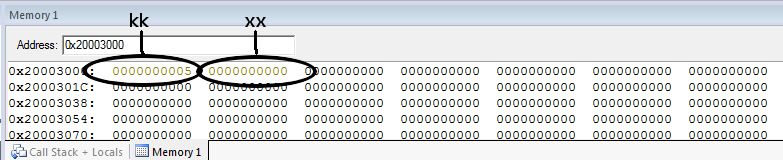
\includegraphics[width=\textwidth,keepaspectratio]{ps2-2_true}
	\caption{The program results for \texttt{PS2-2.s} after the program is run for a TRUE condition. In this case, mm is 30, nn is 20, jj = 10, and cc = 2. Under these conditions, kk is expected to be 5, and xx is expected to be 0. The memory map here indicates that these are, in fact, the resulting values. Therefore, \texttt{PS2-2.s} runs correctly for a TRUE condition.   }
	\label{fig:PS2-2_true}
\end{figure}
\begin{figure}[htbp]
	\centering
	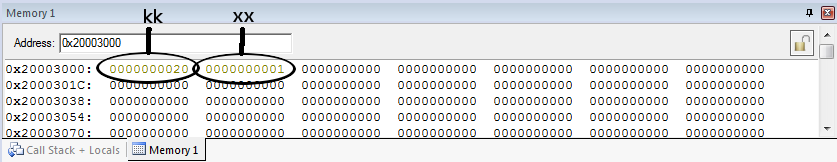
\includegraphics[width=\textwidth,keepaspectratio]{ps2-2_false}
	\caption{The program results for \texttt{PS2-2.s} after the program is run for a FALSE condition. In this case, mm is 30, nn is 10, jj = 10, and cc = 2. Under these conditions, kk is expected to be  20, and xx is expected to be 1. The memory map here indicates that these are, in fact, the resulting values. Therefore, \texttt{PS2-2.s} runs correctly for a FALSE condition.  }
	\label{fig:PS2-2_false}
\end{figure}
\begin{figure}[!ht]
	\centering
	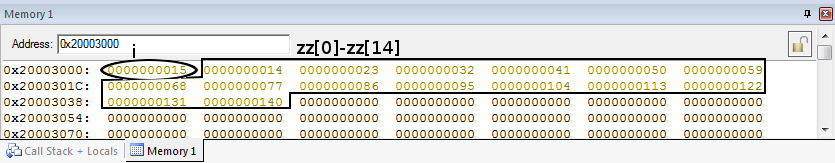
\includegraphics[width=\textwidth,keepaspectratio]{ps2-3_mem}
	\caption{The program results for \texttt{PS2-3.s} after it is executed. The final expected value of i is 15, which is circled. The values for the array, zz, are also circled, and match the expected values, given the arrays used for aa and bb. Because these are the expected values, and because the expected values occur in their expected locations, it can be concluded that \texttt{PS2-3.s} functions properly. }
	\label{fig:PS2-3_mem}
\end{figure}

\newpage
\section*{ Source Programs }
\lstinputlisting{PS2-2.s}
\newpage
\lstinputlisting{PS2-3.s}



%  \begin{figure}[htbp]
%   \centering
%   \includegraphics[width=4.0in,keepaspectratio]{E-Field}
%   \caption{\small{ The E-Field pattern produced by the initial code. }}
%   \label{fig:E-Field}
%   \end{figure}
%  \begin{figure}[htbp]
%   \centering
%   \includegraphics[width=4.0in,keepaspectratio]{Power}
%   \caption{\small{ The normalized power pattern of the system.  }}
%   \label{fig:Power}
%   \end{figure}

\label{end}\end{document}


